%%
%% exam.tex
%% 
%% Made by Roberto Cavada
%% Login   <cavada@localhost.localdomain>
%% 
%% Started on  Sat Dec 16 18:18:21 2006 Roberto Cavada
%% Last on Sat Dec 16 18:26:47 2006 Roberto Cavada
%%


\section{\label{SAP} A simple application}
This section describes the process of creation of a sample
application, from the design with \glade, to the integration of views
and code inside the \mvco Infrastructure.

We want to design and implement a simple application constituted by
only one window, containing two string labels. One label shows a text,
while the other shows the number of characters displayed (i.e. the
length of the string) by the first one. There is also a button the
user can press. By pressing the button, the user can change the
displayed text, and of course this action might change also the
displayed text length accordingly. Figure \ref{EX:f} gives an idea on
how the application should appear.

\begin{figure}[htbp]
\begin{center}
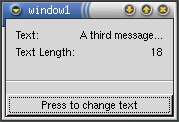
\includegraphics[width=4cm]{figs/png/example}
\caption{\label{EX:f}The sample Application}
\end{center}
\end{figure}

\subsection{\label{GLEX}\glade}
Figure \ref{GL:f} shows \glade and a project named \codename{example}.
The sample \gui has only one top-level window (named
\codename{window1}).

\begin{figure}[here]
\begin{center}
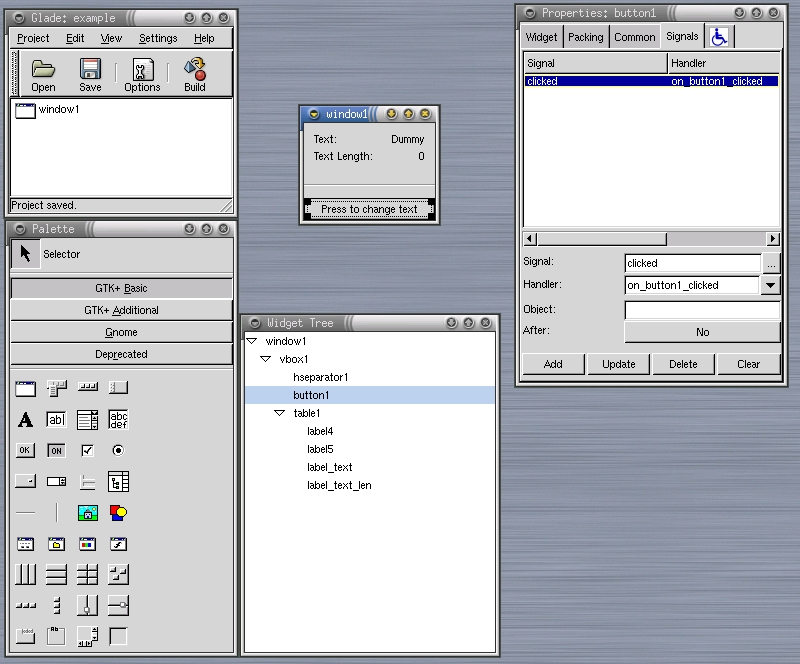
\includegraphics[width=12cm]{figs/png/example_glade}
\caption{\label{GL:f}Designing the example by means of \glade for GTK2}
\end{center}
\end{figure}

The \appl{Widget Tree Window} shows the widgets hierarchy. There are
essentially the three main components (one button and two labels),
grouped inside a set of \emph{containers}, which supplies alignments and
resizing capabilities.

On the right side of Figure \ref{GL:f}, the \appl{Properties Window}
shows that the widget named \codename{button1} has signal
\codename{clicked} associated with function
\codename{on\_button1\_clicked}. This means that the Controller will
have to supply this function in order to handle the \codename{click}
event occurring in \codename{button1}.

\subsection{Implementation}
The implementation is slightly elaborate for this example, because the
goal here is to show how the sample application can be implemented by
using the \mvco Infrastructure.

A basic knowledge of any Object Oriented programming language is
sufficient to understand how this example has been pushed inside the
\mvco framework. On the contrary, a fair knowledge of the Python
language is required in order to understand the code details.

More description section is \ref{DI}.


\subsubsection{View}
In the example, the View is implemented inside the class
\codename{ExampleView} shown below.

{ \codesize 
\begin{verbatim}  
from gtkmvc import View
import os.path

GLADE_NAME = "example.glade"
GLADE_PATH = "./glade" 
GLADE = os.path.join(GLADE_PATH, GLADE_NAME)

class ExampleView (View):
    """The application view. Contains only the main window1 tree."""

    def __init__(self, controller):
        """Contructor, takes the controller instance to perform registration"""
        View.__init__(self, controller, GLADE, "window1")
        return
    pass # end of class
\end{verbatim}}

Global variables named \codename{GLADE*} identify the \glade File to
be used when loading the \gui representation generated by \glade.

Class \codename{ExampleView} extends the generic \codename{View}
class, which performs most of the job, as described above.


\subsubsection{Model}
Class \codename{ExampleModel} is as simple as class
\codename{ExampleView}.  As for \codename{ExampleView}, it extends a
base class of the \mvco Infrastructure, class \codename{Model}.  The
state is represented by a set of possible messages, as well as by the
current message index. The current message index is also an
observable property. A couple of methods are supplied in order to
access the state.

{ \codesize 
\begin{verbatim} 
from gtkmvc import Model

class ExampleModel (Model):
    """The model contains a set of messages
    and an observable property that represent the current message
    index"""

    # Observable property: code for that is automatically generated
    # by metaclass constructor. The controller will be the observer
    # for this property
    __properties__ = {
        "message_index" : -1   # -1 is the initial value
        }

    def __init__(self):
        Model.__init__(self)

        self.messages= ('Initial message',
                        'Another message', 
                        'Another message again',
                        'Model changed again!')
        return

    def get_message(self, index): return self.messages[index]

    def set_next_message(self):
        # this changes the observable property:
        self.message_index = (self.message_index + 1) % len(self.messages)
        return

    pass # end of class

\end{verbatim}
}

Notice the class' variable \codename{\_\_properties\_\_}, which is a
map of (property, value) couples. The base class Model belongs to a
meta-class which automatically searches for observable properties and
generates the needed code to handle the notification.  When the value
of variable \codename{message\_index} changes, all registered
observers will be notified.


\subsubsection{Controller}
Class \codename{ExampleController} contains the \emph{logic} of the
application. The controller handles two signals and the observable
property notification. Signals are the \codename{destroy} event,
invoked when the application quits, and the
\codename{on\_button1\_clicked}, fired when \codename{button1} is
pressed.

{ \codesize 
\begin{verbatim} 
from gtkmvc import Controller
from gtk import mainquit

class ExampleController(Controller):
    """The only one controller. Handles the button clicked signal, and
    notifications about one observable property."""

    def __init__(self, model):
        """Contructor. model will be accessible via the member 'self.model'.
        Registration is also performed."""
        Controller.__init__(self, model)
        return

    def register_view(self, view):
        Controller.register_view(self, view) # Calls the overridden method

        # Connects the exiting signal:
        view.get_top_widget().connect("destroy", mainquit)
        return

    # Signal
    def on_button1_clicked(self, button):
        """Handles the signal clicked for button1. Changes the model."""
        self.model.set_next_message()
        return

    # Observables notifications (value):
    def property_message_index_value_change(self, model, old, new):
        """The model is changed and the view must be updated"""
        msg = self.model.get_message(new)
        
        self.view['label_text'].set_text(msg)
        self.view['label_text_len'].set_text(str(len(msg)))
        return    

    pass # end of class
\end{verbatim}
}

The \codename{destroy} signal is connected when the View registers
itself inside the controller, by using the method override of
\codename{register\_view}.  Method \codename{on\_button1\_clicked}
calls a method inside the model which changes a part of the state
inside the model. Since that part of the state is an observable
property, the associated observer (which is the controller itself) is
notified of the modification, by calling method
\codename{property\_message\_index\_value\_change}. This method
updates the view connected to the controller.

